%
% windowed.tex
%
% (c) 2019 Prof Dr Andreas Müller, Hochschule Rapperswil
%
\section{Gefensterte Fourier-Transformation
\label{section:gefenstert}}
\rhead{Gefensterte Fourier-Transformation}
\begin{figure}
\centering
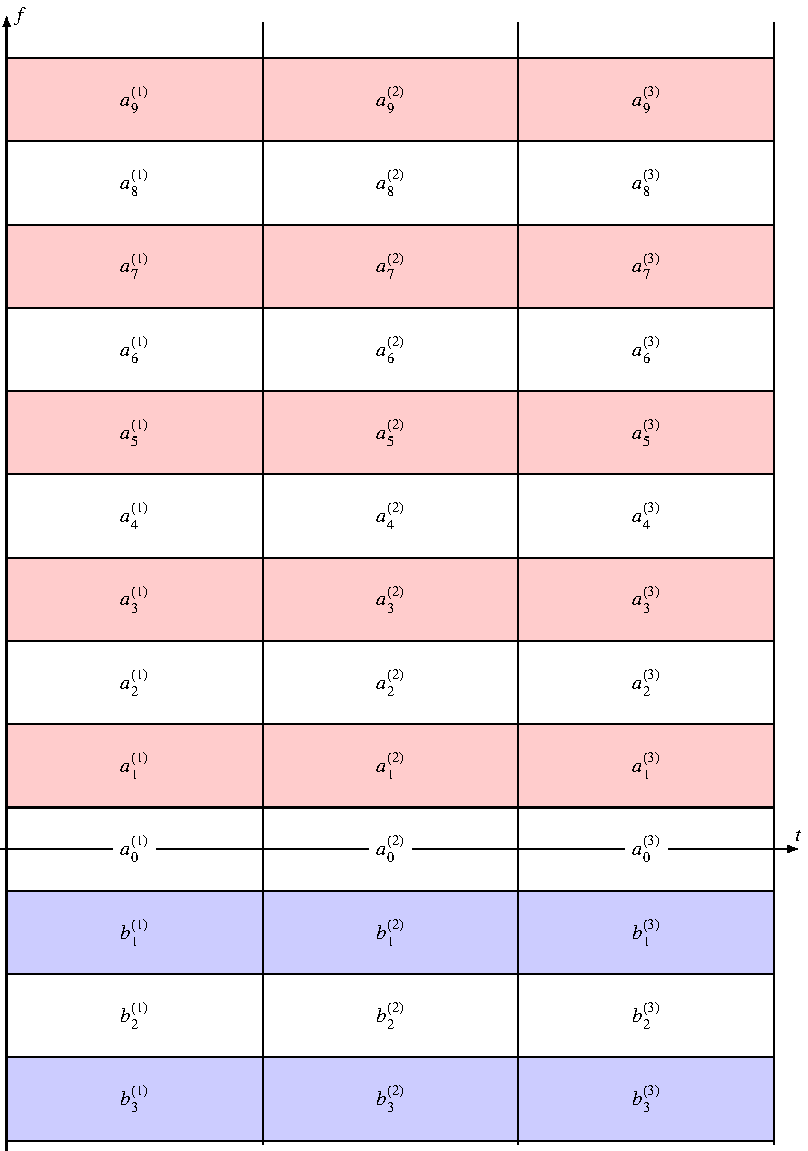
\includegraphics{chapters/2-fourier/images/wft.pdf}
\caption{Aufteilung der Frequenz-Zeit-Ebene für die gefensterte
Fourier-Transformation.
\label{wft:ftplane}}
\end{figure}
Ändert man eine $2\pi$-periodische Funktion in der Umgebung eines Punktes,
dann ändern praktisch alle Fourier-Koeffizienten.
Da die Fourier-Koeffizienten linear von der Funktion abhängen,
reicht es, die Koeffizienten der Änderung zu bestimmen.
Für eine Dirac $\delta$-Distribution im Punkt $t_0$ sind die Koeffizienten
\[
c_k
=
\frac{1}{2\pi} \int_0^{2\pi} \delta(t-t_0) e^{ikt}\,dt
=
\frac{1}{2\pi} e^{ikt_0},
\]
insbesondere ändert jeder Koeffizient um eine Zahl vom Betrag $1/2\pi$.

Die Position einer Störung äussert sich also nur in der Phase, nicht
im Betrag der Störung.
Man könnte sagen, die Information über die Störung ist im Amplitudenspektrum
vollständig delokalisiert.
Diese Eigenschaft der Fourier-Reihen bedeutet, dass transiente Ereignisse
nur sehr beschränkt mit Fourier-Reihen analysiert werden können.

Noch drastischer ist die Situation für die Fourier-Transformation.
Eine $\delta$-Störung in einem Punkt $t_0$ irgendwo auf der reellen Achse
ändert die Transformierte um
\[
\mathcal{\delta_{t_0}}(\omega)
=
\frac{1}{\sqrt{2\pi}} \int_{-\infty}^\infty \delta(t-t_0) e^{-i\omega t}\,dt
=
\frac1{\sqrt{2\pi}} e^{-i\omega t_0}.
\]
Auch in diesem Fall schlägt sich der Ort der Störung nur in der Phase nieder,
nicht in der Amplitude.
Das Amptlitudenspektrum sagt also nichts über die Position der
Störung aus.

Die {\em gefensterte Fouriertransformation} ermöglich, etwas Orts-Information
in die Fourier-Koeffizienten zu rechnen.
Zu diesem Zweck wird das Definitionsgebiet in kleinere Intervalle gleicher
Grösser unterteilt.
In jedem Teil-Interval kann das vorgegebene Signal in eine Fourier-Reihe
entwickelt werden.
Die so ermittelten Fourier-Koeffizienten können sich dann nur auf den Teil
der Funktion im Teilinterval bezienen.
Eine Störung im Punkt $t_0$ wirkt sich nur auf die Fourier-Koeffizienten
für das Interval aus, welches $t_0$ enthält.

Die Unterteilung in kleinere Intervalle erhöht aber auch die Frequenz
der Analysefunktionen.
Wird das Interval $[0,2\pi]$ in $n$ Intervalle unterteilt, dann wird in
jedem Teilinterval mit den Funktionen $e^{inkt}$ für $k\in\mathbb Z$
analysiert.
Die Koeffizienten in den Teilintervalen repräsentieren also ein $n$-mal
grössers Frequenz-Interval, wie dies in Abbildung~\ref{wft:ftplane}
dargestellt ist.

Die Unterteilung in Teilintervalle löst zwar das Problem der Lokalisierung,
ist aber aus anderen Gründen nicht optimal.
Die Berechnung der Fourier-Reihe für das Teilinterval $[2\pi k/n, 2\pi(k+1)/n]$
läuft darauf hinaus, die Fourier-Reihe im Interval $[0,2\pi]$ der Funktion
$f(t) \chi_{[2\pi k/n, 2\pi(k+1)/n]}(t)$
zu berechnen, wobei 
\[
\chi_{[2\pi k/n, 2\pi(k+1)/n]}(t)
=
\begin{cases}
1&\qquad t \in [2\pi k/n, 2\pi(k+1)/n]\\
0&\qquad\text{sonst}
\end{cases}
\]
die charakteristische Funktion des Intervals $[2\pi k/n, 2\pi(k+1)/n]$
ist.
Die Schwierigkeiten rühren daher, dass die charakteristische
Funktion Sprünge aufweist.
Bessere Resultate kann man daher erreichen, wenn man statt einer
charakterisischen Funktion eines Intervals eine glatte Funktion
verwendet, deren Träger das Interval enthält.
Die Wahl dieser sogenannten Fensterfunktion beeinflusst die
Analyse-Koeffizienten, bei sorgfältiger Wahl können aber mindestens
die Glattheits-Eigenschaften der analysierten Funktion und die zugehörigen
Eigenschaften der Koeffizienten erhalten werden.

Unbefriedigend bleibt an der gefensterten Fourier-Transformation aber,
dass für jede Frequenz die gleiche Fensterbreite verwendet wird.
Selbst wenn man also zum Beispiel die Sampling-Rate erhöht und damit
die Auflösung verbessert, kann man Transienten in den
Funktionskoeffizienten trotzdem nur mit der Auflösung der Fensterbreite
lokalisieren.
Eine mögliche Verbesserung besteht darin, die Fensterbreite mit zunehmender
Frequenz zu verkleinern.
Genau dies ist, was die Wavelet-Transformation erreicht, die in
Kapitel~\ref{chapter:haar-wavelet} am Beispiel des Haar-Wavelets und in
Kapitel~\ref{chapter:cwt} in voller Allgemeinheit eingeführt wird.

